\chapter{相关工作}
\label{cha:relatedwork}

股票预测一直是股票投资所关注的一个重点,成功的预测可以为投资者创造巨大的收益。通过人工智能的方法,对股票涨跌进行预测,成为了计算机与金融的交叉领域的研究热点之一。在本章中,我们将介绍股票市场相关知识、新闻事件驱动的股票市场预测和基于方面的情感分析的相关工作。
\section{股票市场相关知识}
股票能否被预测一直是一个值得讨论的话题,在这些讨论中,有效市场假说是非常重要的一个理论。有效市场假说(Efficient Market Hypothesis,简称EMH)是由尤金法玛于1970年整理提出的\cite{fama1970efficient}。这一研究起源于路易斯巴舍利,他使用随机过程的方法,研究股票价格变化的随机性和布郎运动,他认为,过去、现在和未来的事件都 反映在股票市场的价格当中,股价遵循公平游戏模型。尤金法玛总结了前人的理论和实证,提出了有效市场假说,包括以下三个要点。
\begin{itemize}
    \item 市场中每个人都是理性的,市场中每支股票都处于这些理性人的监视之下,他们每天对股票价格进行分析和预测,并谨慎地在风险与收益之间进行取舍;
    \item 股票价格反映了这些理性人的供求平衡,买方等于卖方;
    \item 股票的价格反映了全部的可获取信息,当有新的消息出现时,股票价格会迅速地调整到合理的价位。
\end{itemize}
有效市场假说意味着“天下没有免费的午餐”,人们无法在有效市场中获得超额收益。然后有效市场假说也不一定完全正确,不是每个交易者都是完全的理性人,信息也并不一定在每个时刻都发生效果。有效市场假说被越来越多地证明不符合现实。

有效市场假说面临许多理论挑战:
\begin{itemize}
	\item 投资者并非完全理性的;
	\item 投资者不仅偶然偏离理性,而是经常以同样的方式偏离理性;
	\item 套利者不会完全消除非理性投资者的错误对价格的影响。
\end{itemize}
随着人工智能技术的发展,之前的研究表明,股票价格在某种程度上是可以被预测的。
\begin{figure}[ht]
	\centering 
	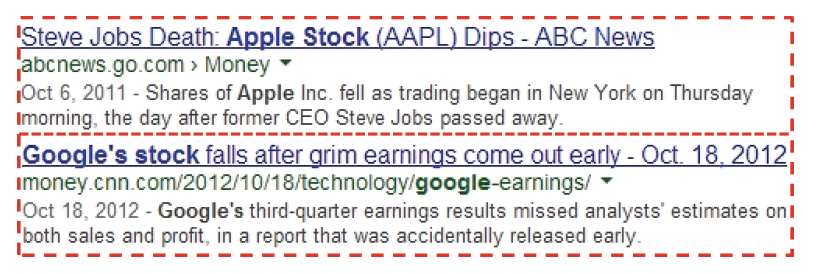
\includegraphics[width=0.8\linewidth]{NEWS-EVENT.png}
	\caption{苹果公司和谷歌公司相关新闻两则}
	\label{fig:stock-event}
\end{figure}
如图\ref{fig:stock-event}显示了两条金融新闻。在苹果前CEO乔布斯去世后,苹果的股票价格开始下跌;同时,在谷歌的收入报告公布后,由于收入不理想,谷歌的价格开始下跌。从中可以看出,新闻事件对股票市场有着重要的影响。
%另一方面,分型市场假说(Fractal Market Hypothesis,简称FMH),建立在非线性动力系统之上,利用流动性和投资起点很好地解释了有效市场假说无法理解的市场现象。分形市场假说主要内容包括:
%\begin{itemize}
%    \item 市场中有许多水平不同的投资者,投资者水平不同会对其行为产生重大影响;
%    \item 信息对不同水平的投资者影响不同,频繁交易的交易员会更加关注技术分析信息。而市场中基本分析投资者更关注对股票价格进行价值评估。在分型市场假说中,技术分析和基本分析都适用,但其影响与投资者的水平相关;
%    \item 市场稳定在于流动性的保持,只有市场处在不同投资水平的众多投资者组成时,流动性才能得以实现;
%    \item 价格反映了市场中的基于技术分析的短期评估和基于基本分析的价值评估;
%    \item 如果股票市场与整体经济循环无关,则市场本身并无长期趋势可言,交易、流动性和短期信息将在市场中起决定作用。
%\end{itemize}
%与有效市场假说不同的是,分形市场假说认为信息的重要性是按照不同投资者来判断的。不同投资者对信息的判断不同,信息的传播并非均匀扩散的。价格并不能反映全部己有的信息,只是反映 与投资者相对应的信息的重要性。有效市场是分形市场的一个特例,分形市场假说拓展了有效市场的含义,更广泛、准确地刻画了市场。
% \begin{table}[ht]
%     \centering
%     \caption{有效市场假说和分形市场假说的对比}
%     \label{tab:compare}
%     \begin{tabular}{|l|l|l|}
%         \hline 
%         特征 & 有效市场理论 & 分形市场理论  \\ 
%         市场特征 & 线性孤立系统 & 非线性、开放、耗散系统 \\ 
%         均衡状态 & 均衡 & 允许非均衡 \\ 
%         系统复杂性 & 简单系统 & 具有分形、混沌等特性的复杂系统 \\ 
%         反馈机制 & 无反馈 & 正反馈 \\ 
%         对信息的反应 & 线性因果关系 & 非线性因果关系 \\ 

%     \end{tabular}
% \end{table}
\section{新闻驱动的股票预测}

股票市场能否被预测一直都是一个值得讨论的问题。大量经验性的研究表明,股价是可以被预测的~\cite{bollen2011twitter,ding2014using,ding2015deep,ding2016knowledge-driven}。新闻事件能够影响交易员的决定,而交易员的交易会影响股票的价格。因此,新闻事件可以影响股票价格的变动。

\subsection{推特情绪预测指数涨跌}
依照行为金融学的观点,情绪可以影响个体的行为和决定。为验证这一规律是否能扩展到大规模群体上,研究者研究了大规模的推特情绪状态与道琼指数(Dow Jones Industrial Average, DJIA)的相关性~\cite{bollen2011twitter}。他们使用两种情绪分析工具来分析每天推特的文本内容:OpinionFinder~\cite{Wilson2005OpinionFinder}和GPOMS(Google-Profile of Mood States)~\cite{Spielberger1972Profile}。

\subsubsection{OpinionFinder}
OpinionFinder是一个公开的软件工具\footnote{http://mpqa.cs.pitt.edu/opinionfinder/opinionfinder\_2/},用于提取句子级的主观情绪极性(积极或消极)。

预处理阶段,利用Standford提供的词性标注工具,对输入进行句子分割和词性标注;然后从中选取主观的能反应情绪的词语;然后基于朴素贝叶斯方法和情感词库,对文本进行分类。

\subsubsection{GPOMS}

GPOMS是原作者自己提出的一款情感分析工具,它使用了Profile of Mood States(POMS-bi),一个由严格审查的心理学仪器提供的词库。为了使这一词库可以应用于推特情绪的分析,作者对词库进行了扩充。推特内容的情感被细分为了六类,包括冷静(Calm),警惕( Alert),肯定( Sure),重要( Vital),和善( Kind)和高兴(Happy)。

利用上述两种工具,他们将推特情感分为六类,包括冷静(Calm),警惕( Alert),肯定( Sure),重要( Vital),和善( Kind)和高兴(Happy)。然后,他们利用格兰杰因果分析(Granger Causality Analysis)和自组织模糊神经网络(Self-Organizing Fuzzy Neural Network),来验证利用上述两种工具得到的情感时间序列是可以用来预测道琼指数的收盘价。他们预测道琼指数收盘价的涨跌的准确率达到了87.6\%。

这一研究表明,网络信息的情感极性是可以用来预测股票市场的变动的。

\subsection{结构化的事件表示}

为了解决新闻事件驱动的股票市场预测,研究者提出事件的结构化表示~\cite{ding2014using}。以往的新闻事件驱动的股票预测,往往使用浅层特征,比如词袋特征(Bag of Words),命名实体,名词等,无法获取实体关系信息。

他们提出结构化的事件表示,使用一个四元组$(O_1,P,O_2,T)$来表示事件,其中$P$表示动作(Action),$O_1$表示动作的发起者(Actor),$O_2$表示动作的作用者(Object),$T$表示动作发生的时间(Time)。比如,“2013年9月3日,微软同意以7.2亿美元的价格收购诺基亚的手机部门”这一新闻事件可以表示为(Actor=微软,Action=收购,Object=诺基亚手机部门,Time=2013年9月3日)。

具体地,研究者们使用依存关系分析器提取句子的结构,选取动词$P$(Action),然后将其左侧最近的名词作为动作的发起者$O_1$,将其右侧最近的名词作为动作的作用者$O_2$。下面我们简单介绍词袋特征和结构化的事件表示方法。

\subsubsection{词袋模型}

% 在信息检索中,词袋模型(Bag of Words Model)假定对于一个文本,忽略其词序和语法,句法,将其仅仅看做是一个词集合,或者说是词的一个组合,文本中每个词的出现都是独立的,不依赖于其他词是否出现,或者说当这篇文章的作者在任意一个位置选择一个词汇都不受前面句子的影响而独立选择的。
在这里,使用经典的TFIDF(Term Frequency–Inverse Document Frequency,词频与逆向文档频率)值作为词袋特征。TFIDF被用来评估某一字词对于一个文件集或一个语料库的重要程度。字词的重要性随着它在文件中出现的次数成正比增加,但同时会随着它在语料库中出现的频率成反比下降。

\subsubsection{结构化事件表示}

前面已经提到用一个四元组$(O_1,P,O_2,T)$来表示事件。为了解决数据稀疏性的问题,使用退化的特征,即使用元素的合并作为事件的表示,即$(O_1,P,O_2,O_1+P,P+O_2,O_1+P+O_2)$。具体地,对事件四元组(Microsoft,buy,Nokia's mobile phone business)可以表示为(\#arg1=Microsoft,\#arg2=buy,\#arg3=Nokia's mobile phone,\#arg4=Microsoft buy,\#arg5=buy Nokia's mobile phone business,\#arg6=Microsoft buy Nokia's mobile phone business)。然后,为每个字符串生成一个特定的向量表示,这几个字符串拼接起来作为事件的表示。因为动作、动作发起者、动作作用者的数据非常稀疏,这里去掉时态、复数等特征,并将动作转换为动作的类别,以减少数据的稀疏性。

同时,这里还使用了线性和非线性的模型来解决新闻事件驱动的股票预测问题。线性模型选取的是SVM(Supported Vector Machine,支持向量机)模型,非线性模型选取的是三层神经网络。

实验结果显示,预测标普500的准确率达到了60\%,单支股票预测的准确率超过70\%。

\subsection{深度学习与新闻驱动的股票预测}

前面所提到的结构化的事件表示方法,使用的是单词向量的拼接。为改进这一方法,研究者提出用一个神经网络来学习事件的表示。图~\ref{fig:neural-tensor-network}显示了提取事件特征所使用的网络结构。

\begin{figure}[ht]
    \centering 
    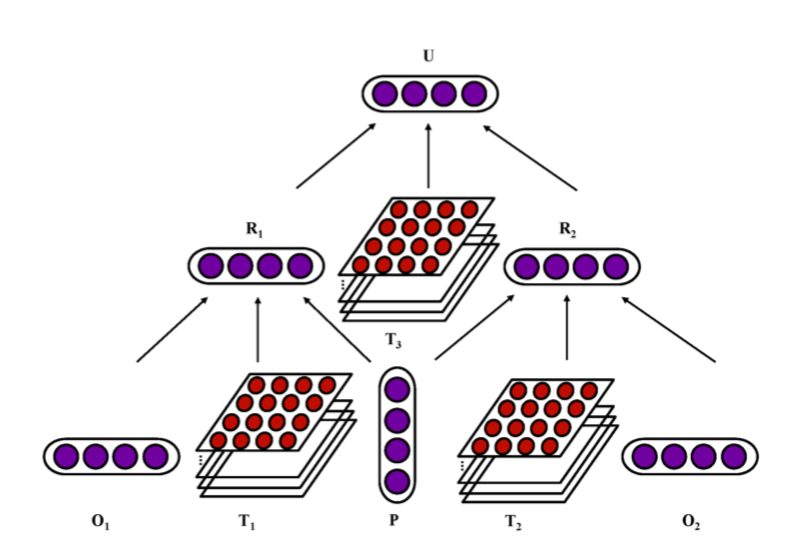
\includegraphics[width=0.5\linewidth]{neural-tensor-network.png}
    \caption{Neural Tensor Network结构}
    \label{fig:neural-tensor-network}
\end{figure}

这里用到的事件表示方法,与前面提到的四元组结构化表示一致。不同的是,不再使用退化的特征,而是使用一个神经网络Neural Tensor Network来训练学习得到事件的向量化表示。具体地,Actor、Action、Object均被表示为一个向量$O_1$、$P$、$O_2$。然后,利用矩阵$T_1$融合Actor~$O_1$和Action~$P$得到$R_1$,利用矩阵$T_2$融合Action~$P$和Object~$O_2$得到$R_2$,利用矩阵$T_3$融合$R_1$和$R_2$得到事件最终的向量表示。

模型上,这里用到了卷积神经网络。图~\ref{fig:cnn}显示了模型的结构。上面得到的事件的向量化表示被用来当作短期事件的表示,然后利用CNN和max pooling层得到中期和长期的事件表示。将短期、中期、长期的事件表示拼接起来,并通过两层神经网络预测得到最终的预测结果。

\begin{figure}[ht]
    \centering 
    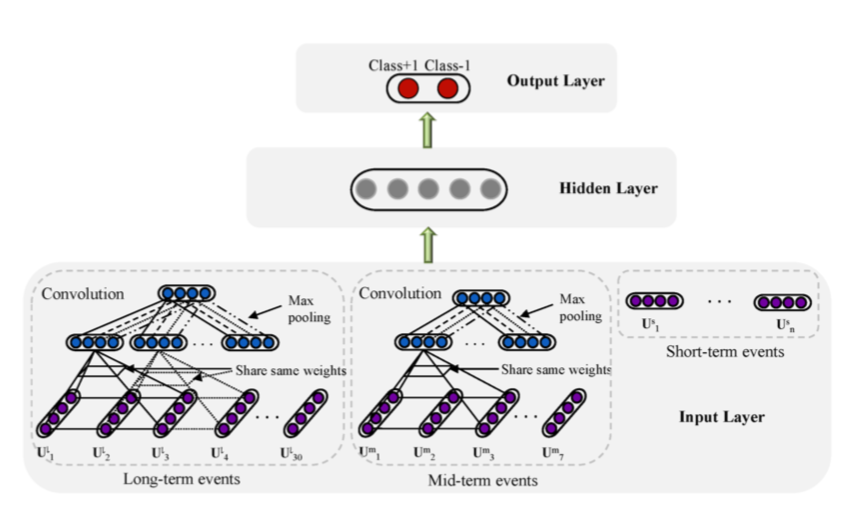
\includegraphics[width=0.5\linewidth]{CNN.png}
    \caption{基于CNN的预测模型结构}
    \label{fig:cnn}
\end{figure}

相比于之前的方法,利用神经网络学习得到的事件表示,可以将标普500的预测准确率提升将近6\%。

这些新闻事件驱动的股票预测表明,新闻事件与股票的变动是相关的,新闻事件可以用来作为股票预测的依据。但是,无论是利用OpinionFinder等工具的方法,还是结构化、向量化的表示,都忽视了新闻文本中的一些细节信息。随着自然语言处理技术的发展和词向量的提出,直接将新闻文本作为事件的表示,将股票预测转化为文本分类成为了更为合适的处理方式。

\section{基于方面的情感分析}

基于方面的情感分析旨在提取某个句子对某一方面或目标的情感极性~\cite{pontiki2014semeval-2014}。比如,“这家餐厅的菜很好吃,但服务太差了”对“食物”方面的情感是积极的,对“服务”方面的情感是消极的。基于方面的情感分析又细分为对某一方面的情感分析和对某一目标的情感分析。对某一方面的情感分析(Aspect-Category Sentiment Analysis)中,方面可能是一个抽象的概念,并不一定在句子当中出现;而对某一目标的情感分析(Aspect-Term Sentiment Analysis or Target-oriented Sentiment Analysis)中,目标一定是句子中的某一个词。随着自然语言处理技术的发展,研究者们提出了许多深度学习的模型来解决这一问题。

\subsection{ATAE-LSTM}

\begin{figure}[ht]
    \centering 
    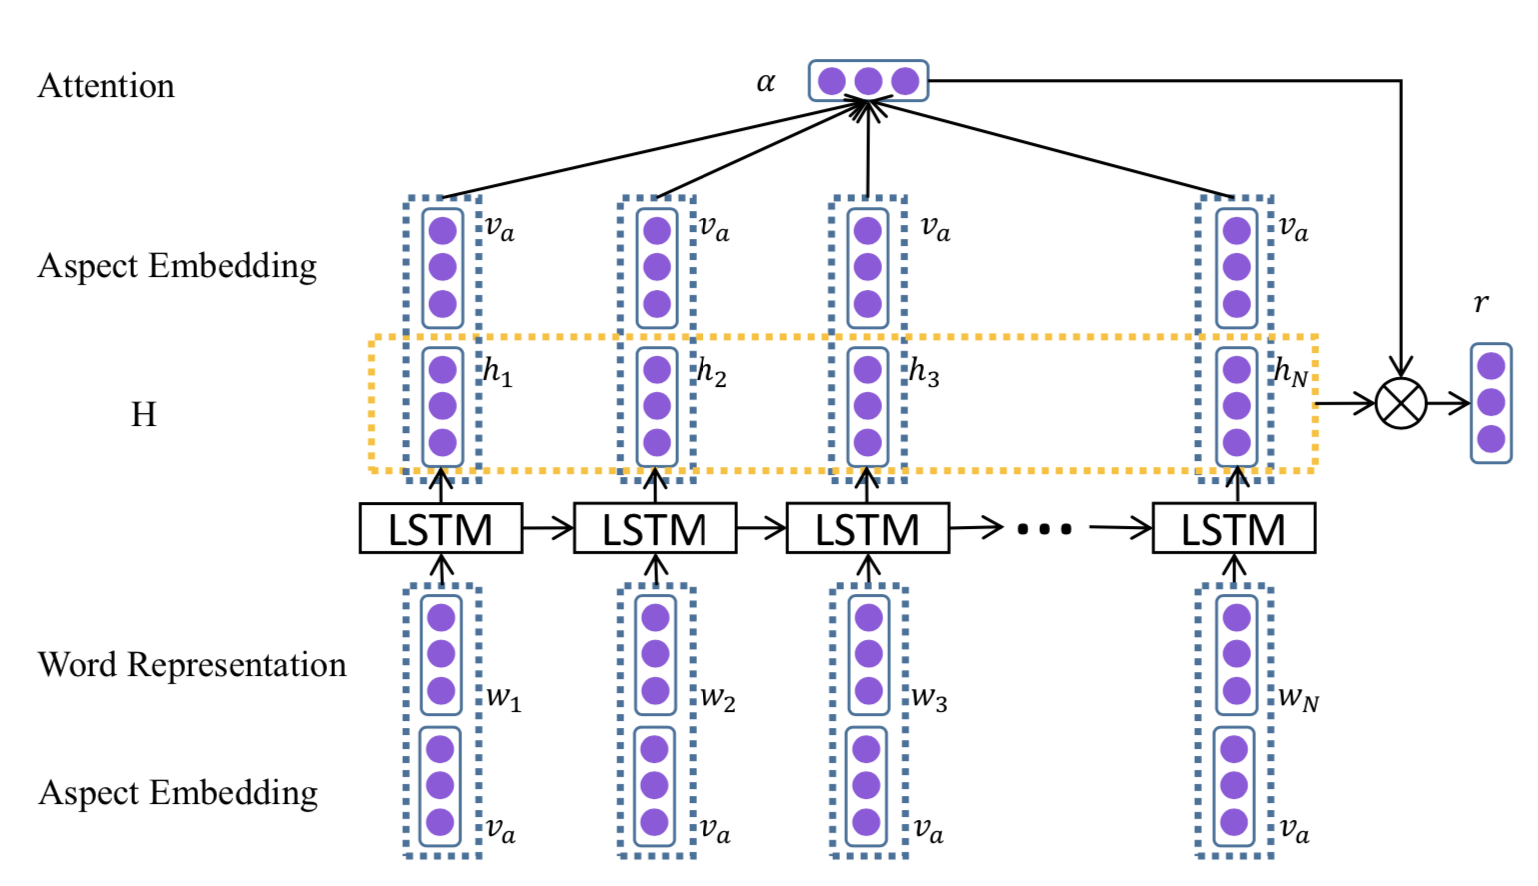
\includegraphics[width=0.8\linewidth]{atae-lstm.png}
    \caption{ATAE-LSTM模型结构}
    \label{fig:atae-lstm}
\end{figure}

ATAE-LSTM(Attention-based LSTM with Aspect Embedding)~\cite{wang2016attention-based}是一个结合了LSTM\cite{hochreiter1997long}和attention机制的模型。与直接使用LSTM模型相比,图~\ref{fig:atae-lstm}显示了ATAE-LSTM模型的结构。ATAE-LSTM使用了attention机制,当输入不同的aspect(方面)时,会对句子的不同部分有不同的侧重。因为aspect(方面)起着非常关键的作用,ATAE-LSTM模型用两种方式使用了aspect的信息:一个是在计算attention的加权和时,把aspect的信息和句子的隐式信息表示拼接起来;另一个是把aspect表示和输入单词向量拼接起来。ATAE-LSTM模型既可以处理对某一方面的情感分析(Aspect-Category Sentiment Analysis),也可以处理对某一目标的情感分析(Aspect-Term Sentiment Analysis or Target-oriented Sentiment Analysis)。ATAE-LSTM相比于LSTM模型,考虑了aspect的信息,引入了attention的机制。

\subsection{IAN}

\begin{figure}[ht]
    \centering
    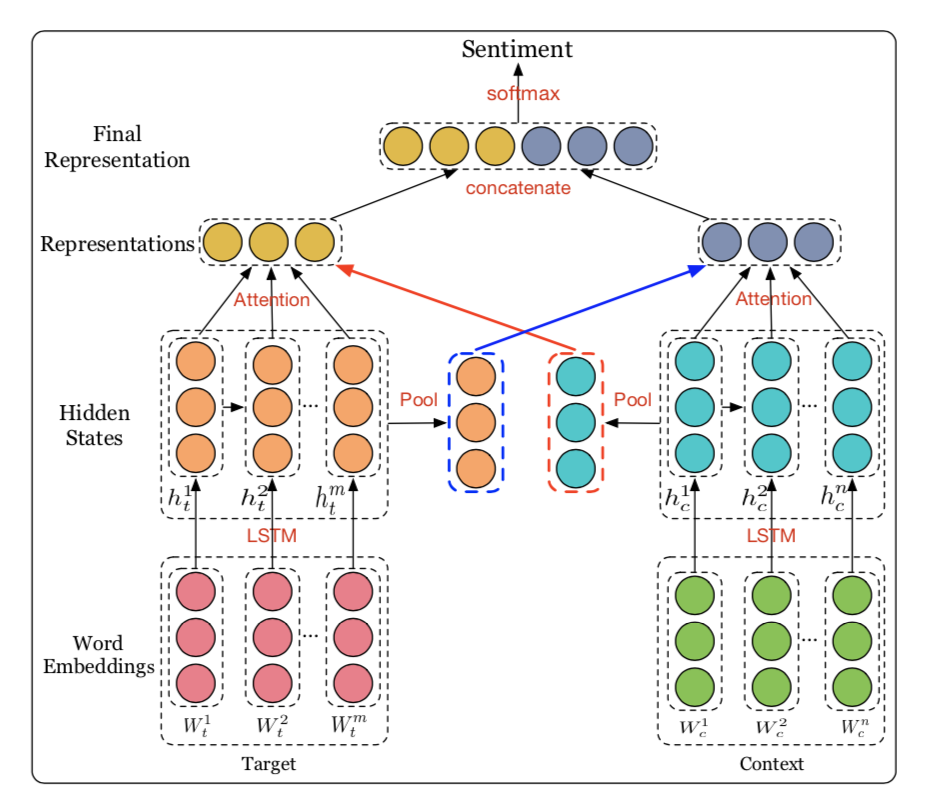
\includegraphics[width=0.7\linewidth]{ian.png}
    \caption{IAN模型结构}
    \label{fig:ian}
\end{figure}

在对某一目标的情感分析(Aspect-Term Sentiment Analysis or Target-oriented Sentiment Analysis)中,目标(target)可能由多个词组成。在针对不同的句子时,目标中的单词也可能发挥着不同的重要性。因此,IAN(Interactive Attention Networks)~\cite{ma2017interactive}提出目标的表示和句子的表示都需要通过交互式地学习得到。图~\ref{fig:ian}显示了IAN模型的结构。

首先,IAN使用LSTM处理句子和目标,得到了句子和目标的隐式向量表示。然后,通过均值pooling的方式,得到句子和目标的表示,并以此计算attention的权重,对句子和目标中的隐式表示进行加权求和。最后,将句子和目标的加权和结果拼接,作为整个输入的表示。IAN相比于ATAE-LSTM,使用了交互式的attention机制,同样考虑了目标中不同单词的不同重要性。

\subsection{BILSTM-ATT-G}

\begin{figure}[ht]
    \centering 
    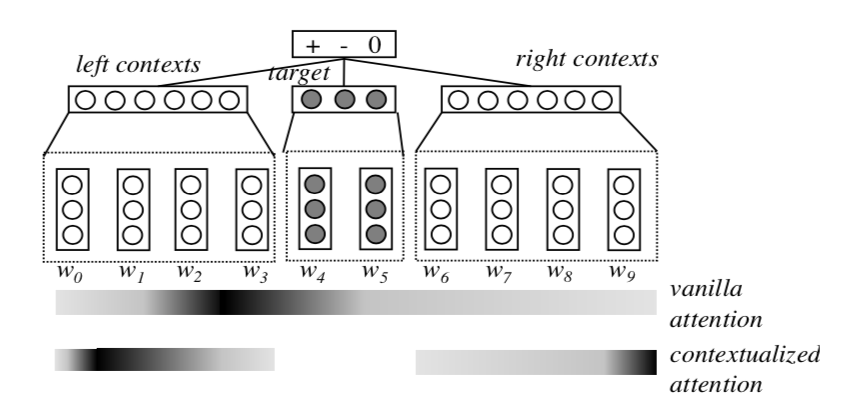
\includegraphics[width=0.8\linewidth]{bilstm-att-g.png}
    \caption{BILSTM-ATT-G模型结构}
    \label{fig:bilstm-att-g}
\end{figure}

在处理对某一目标的情感分析(Aspect-Term Sentiment Analysis or Target-oriented Sentiment Analysis)时,BILSTM-ATT-G(BiLSTM with Attentional Gates)~\cite{liu2017attention}除了考虑不同单词的重要性,还考虑了句子不同部分的重要性。图~\ref{fig:bilstm-att-g}显示了BILSTM-ATT-G的结构。它用目标将句子分成了左边、右边和目标三部分。首先,它使用与上面提到的简单attention模型来处理句子的左边部分、右边部分和目标;然后,利用attention模型的输出和最后一个隐层表示来计算一个门,并通过这个门对不同的部分的结果加权求和。这一方法对模型的效果有巨大的提升。从中可以看出,句子中不同的部分有着不同的重要性,gate方法可以很好地学习到这种重要性。

\subsection{GCAE}

\begin{figure}[ht]
    \centering 
    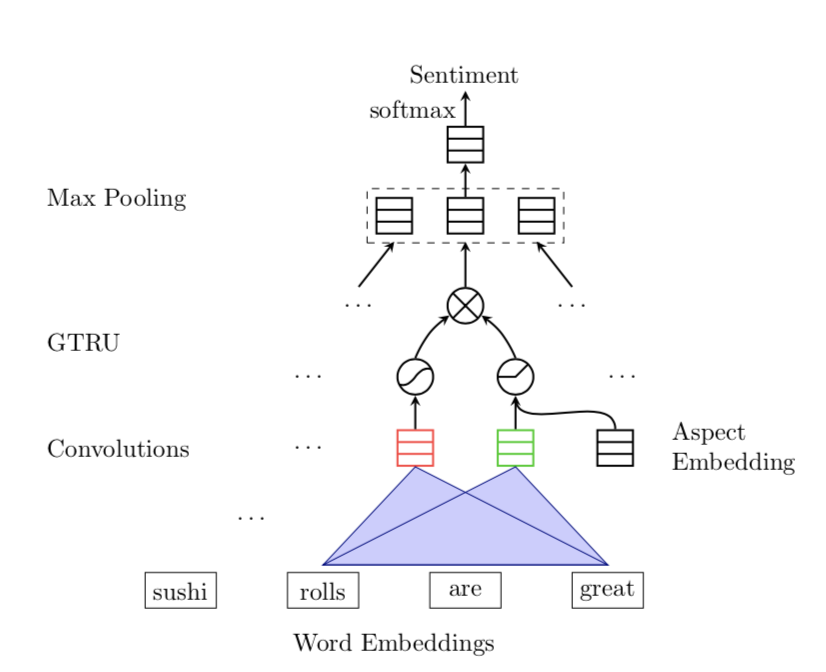
\includegraphics[width=0.8\linewidth]{gcae.png}
    \caption{GCAE模型结构}
    \label{fig:gcae}
\end{figure}

在前面所提到的模型中,LSTM等循环结构被用来处理单词的向量,得到句子的隐式表示。由于LSTM难以并行化,且当句子长度较长时训练困难,GCAE(Gated Convolutional Network with Aspect Embedding)开始尝试用CNN\cite{krizhevsky2012imagenet,grefenstette2014convolutional}解决处理句子。图~\ref{fig:gcae}显示了GCAE模型的结构。首先,GCAE用一维卷积处理句子输入,得到了句子的表示;然后对句子的单词和target的单词进行卷积,得到控制门;将二者相乘,得到了输入的表示。为了从不同粒度处理句子的特征,GCAE用到了多尺度的卷积,即使用了多个不同卷积核大小的卷积,并将它们的结果拼接起来。

\subsection{Memnet}

\begin{figure}[ht]
    \centering 
    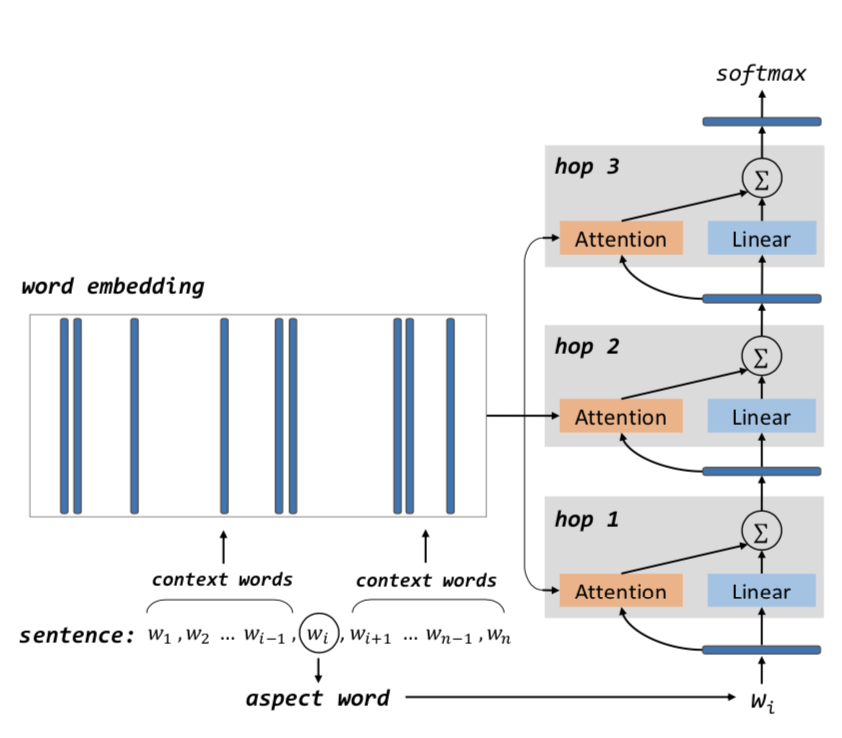
\includegraphics[width=0.7\linewidth]{memnet.png}
    \caption{Memnet模型结构}
    \label{fig:memnet}
\end{figure}

除了attention机制和gate方法,memory network~\cite{Weston2014Memory}也被应用到基于方面的情感分析中来。Memory network是一项机器学习技术,在问答系统中取得了优秀的表现~\cite{Weston2014Memory,Sukhbaatar2015End}。图~\ref{fig:memnet}显示了Memnet模型的结构。Memnet是一个多层结构。首先,它把单词的向量表示当作记忆单元,把目标单词的均值当作初始query;每层是一个attention的结构,上一层的结果作为下一层的query;各层结果之和作为最终的输出。Memnet利用了多层attention结构,它很好地解决了长期依赖的问题。但是,Memnet也存在一些问题:它直接使用单词的表示作为记忆单元,使得难以处理词组的信息;attention方法对单词的顺序不敏感,这样忽视了单词的时序信息。Memnet在处理需要推断、否定和比较的问题时遇到了困难。

\subsection{RAM}

\begin{figure}[ht]
    \centering 
    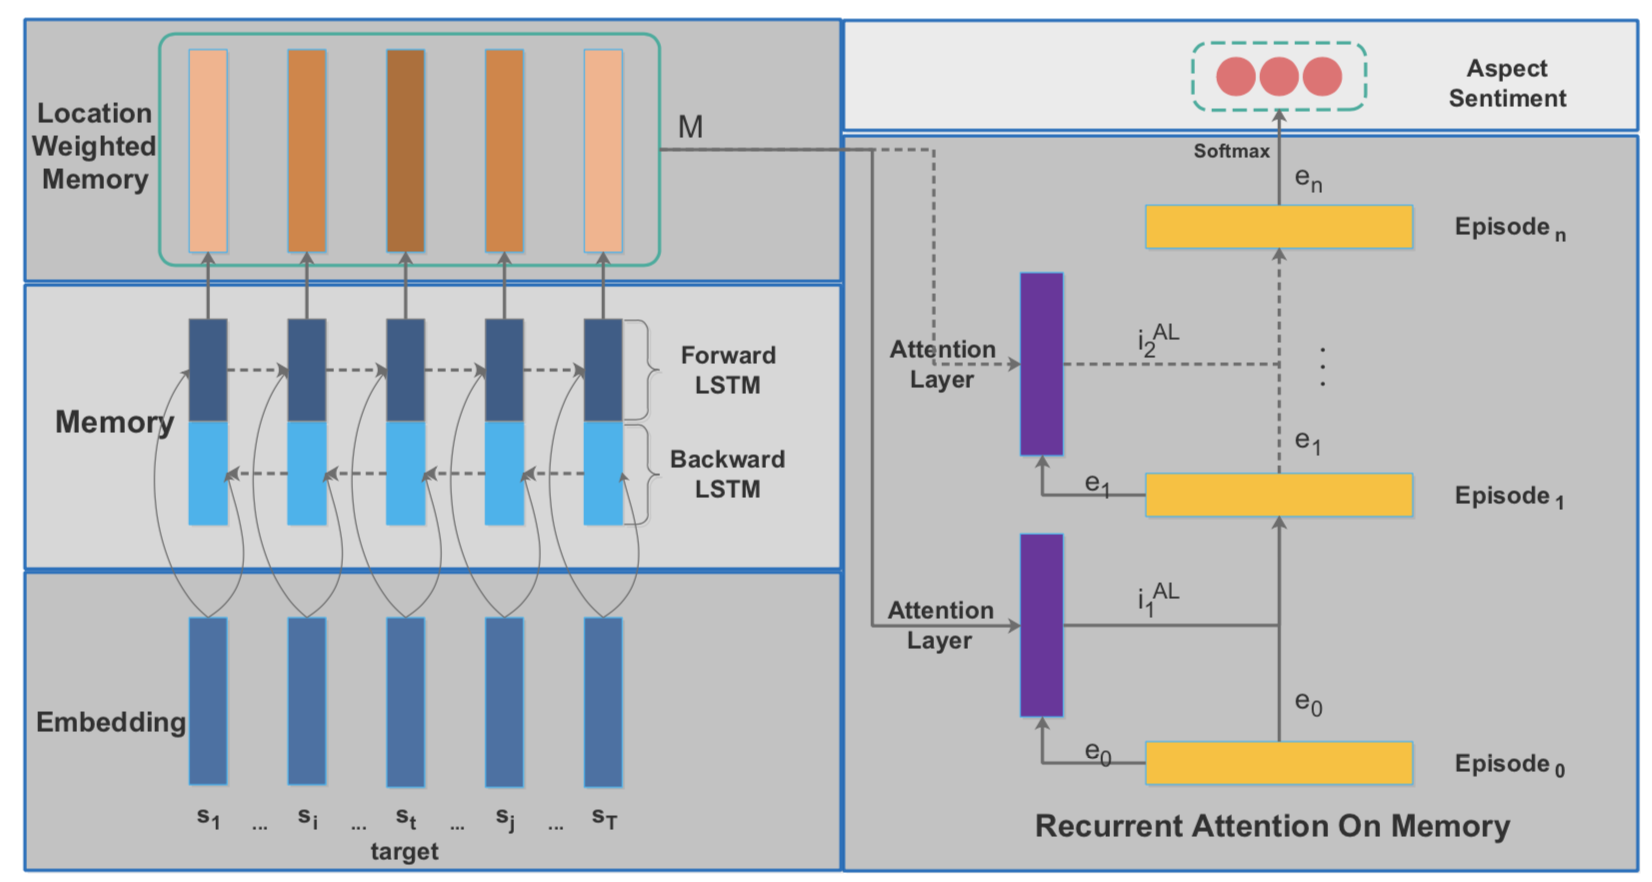
\includegraphics[width=0.7\linewidth]{ram.png}
    \caption{RAM模型结构}
    \label{fig:ram}
\end{figure}

针对Memnet的一些缺陷,RAM(Recurrent Attention Network)~\cite{Al2017Deep}。图~\ref{fig:ram}显示了RAM模型的结构。为了解决Memnet不善处理词组的问题,它使用双向LSTM来处理句子单词,得到了结合上下文的句子表示,并以此作为记忆单元;为了使模型具备一定的推断、否定和比较的能力,它不再简单地将上一层的输出作为下一层的query,而是利用一个\cite{cho2014learning}单元,得到下一层的query;同时,为了弥补Memnet不带有时序信息的问题,它引入了位置权重,使得与目标更近的单词权重更大。

\subsection{TNet}

\begin{figure}[h]
	\centering%
	\begin{subfigure}{0.5\textwidth}
		\centering
		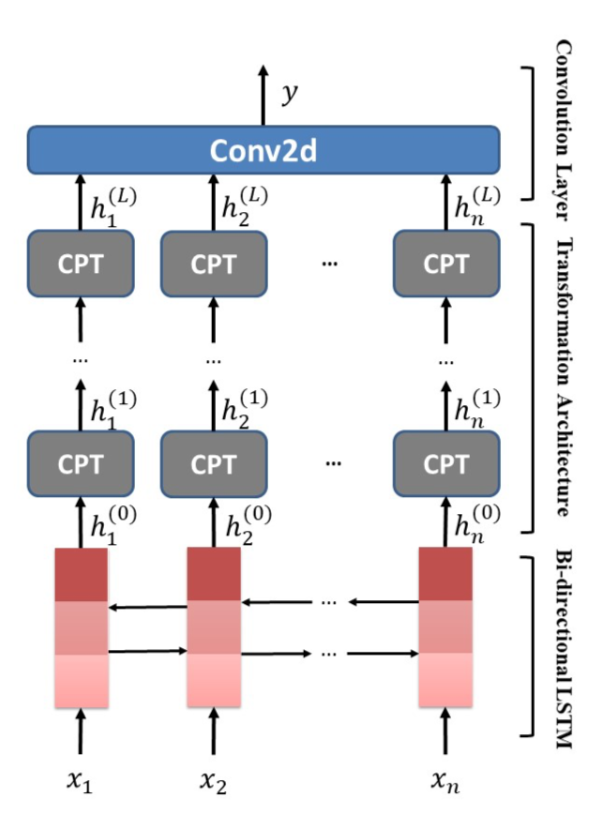
\includegraphics[width=0.5\textwidth]{tnet.png}
		\caption{整体结构}
	\end{subfigure}%
%	\hspace{4em}%
	\begin{subfigure}{0.5\textwidth}
		\centering
		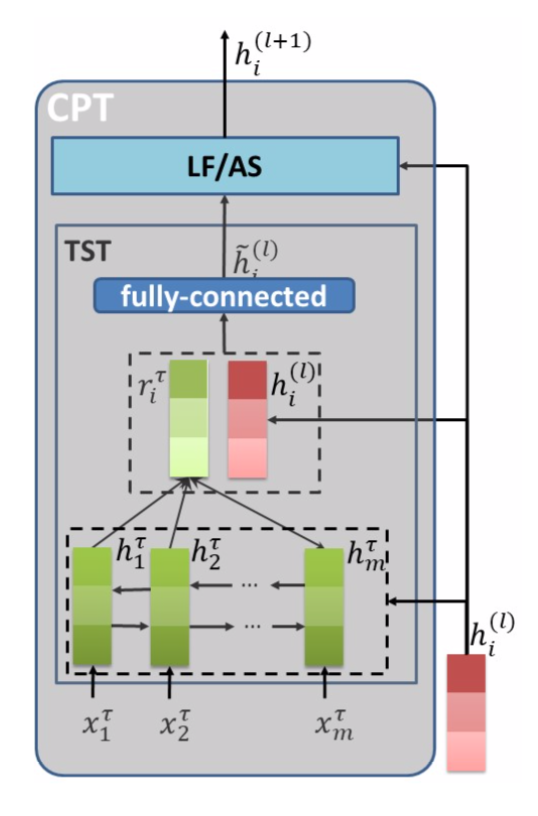
\includegraphics[width=0.5\textwidth]{cpt.png}
		\caption{CPT模块}
	\end{subfigure}
	\caption{TNet模型}
	\label{fig:tnet}
\end{figure}

TNet(Transformation Network)~\cite{Xin2018Transformation}集成了众多的技术,在多个公开数据集上取得了最佳的结果。图~\ref{fig:tnet}左图显示了TNet模型的结构。首先,它使用双向LSTM处理句子单词,得到结合上下文的表示,并以此作为记忆单元;然后,利用一个多层结构处理记忆单元;最后,利用二维卷积得到最终的句子表示。具体地,在每一层中,使用一个名为CPT(Context-Preserving Transformation)的结构,其结构如图~\ref{fig:tnet}右图所示。在CPT结构中,对每个句子中的单词,使用attention方法求得与句子单词相关的目标表示,将其与上一层的记忆单元通过一个单层映射得到下一层的记忆单元。同时,TNet还使用了更加复杂的位置权重。